%!TEX root = ../hutbthesis_main.tex

\chapter{模型校核、性能评价方法与工况设计}

\section{基准工况自检与模型校核}

进行多工况仿真分析之前，要先针对着陆控制动力学模型进行基准工况自检、模型校核工作，目的是确保后续结果具备可比性与可信性。本文把平坦地形、正常模式、无初始侧偏、无额外航向误差选作基准工况。其参数设定如下：初始离地高度为120
ft，初始速度是72 kts，初始下降率为-250 fpm，跑道距离为2200
ft，下滑角为3.0$^\circ$，目标接地点设定在跑道阈值后120
ft处，同时开启约束保护逻辑。

依据仿真结果可知，在基准工况时飞行器能够沿着预定的下滑轨迹实现稳定下降，其离地高度随着时间持续减小，速度维持在安全范围之内，俯仰角、滚转角的变化较小，这表明该模型在纵向控制还有侧向控制方面整体比较协调。当进入着陆末段之后，系统能够及时从进近阶段转换至拉平阶段，并且在接地区域优先执行稳定接地逻辑，没有出现明显的轨迹突变或者状态发散情况。已有结果显示，在该工况下仿真时长大约是17.15
s，末段离地高度约为4.60 ft，末段速度约为71.80
kts，末段俯仰角约为-1.28$^\circ$，末段滚转角约为-2.28$^\circ$。这些数据表明模型在标准条件下运行稳定，能够满足后续复杂工况分析的需求。

模型校核主要有三个方向：其一为轨迹合理性，也就是查看飞行器能否顺着预定下滑路径持续靠近跑道，其二是状态边界合理性，即检验速度、下沉率、姿态角、侧偏量是否处于合理区间，其三是阶段切换合理性，即核查系统是否能够在适宜的高度和距离进入flare阶段，并在近地区域维持以稳定接地为主的控制策略。精确着陆研究通常觉得，着陆控制模型是否可靠，既体现在轨迹能否闭合，也体现在关键状态量是否处在可接受窗口内。所以，本文经由基准工况的自检来确认模型拥有后续多工况比较的基本条件。

\begin{figure}[H]
\centering
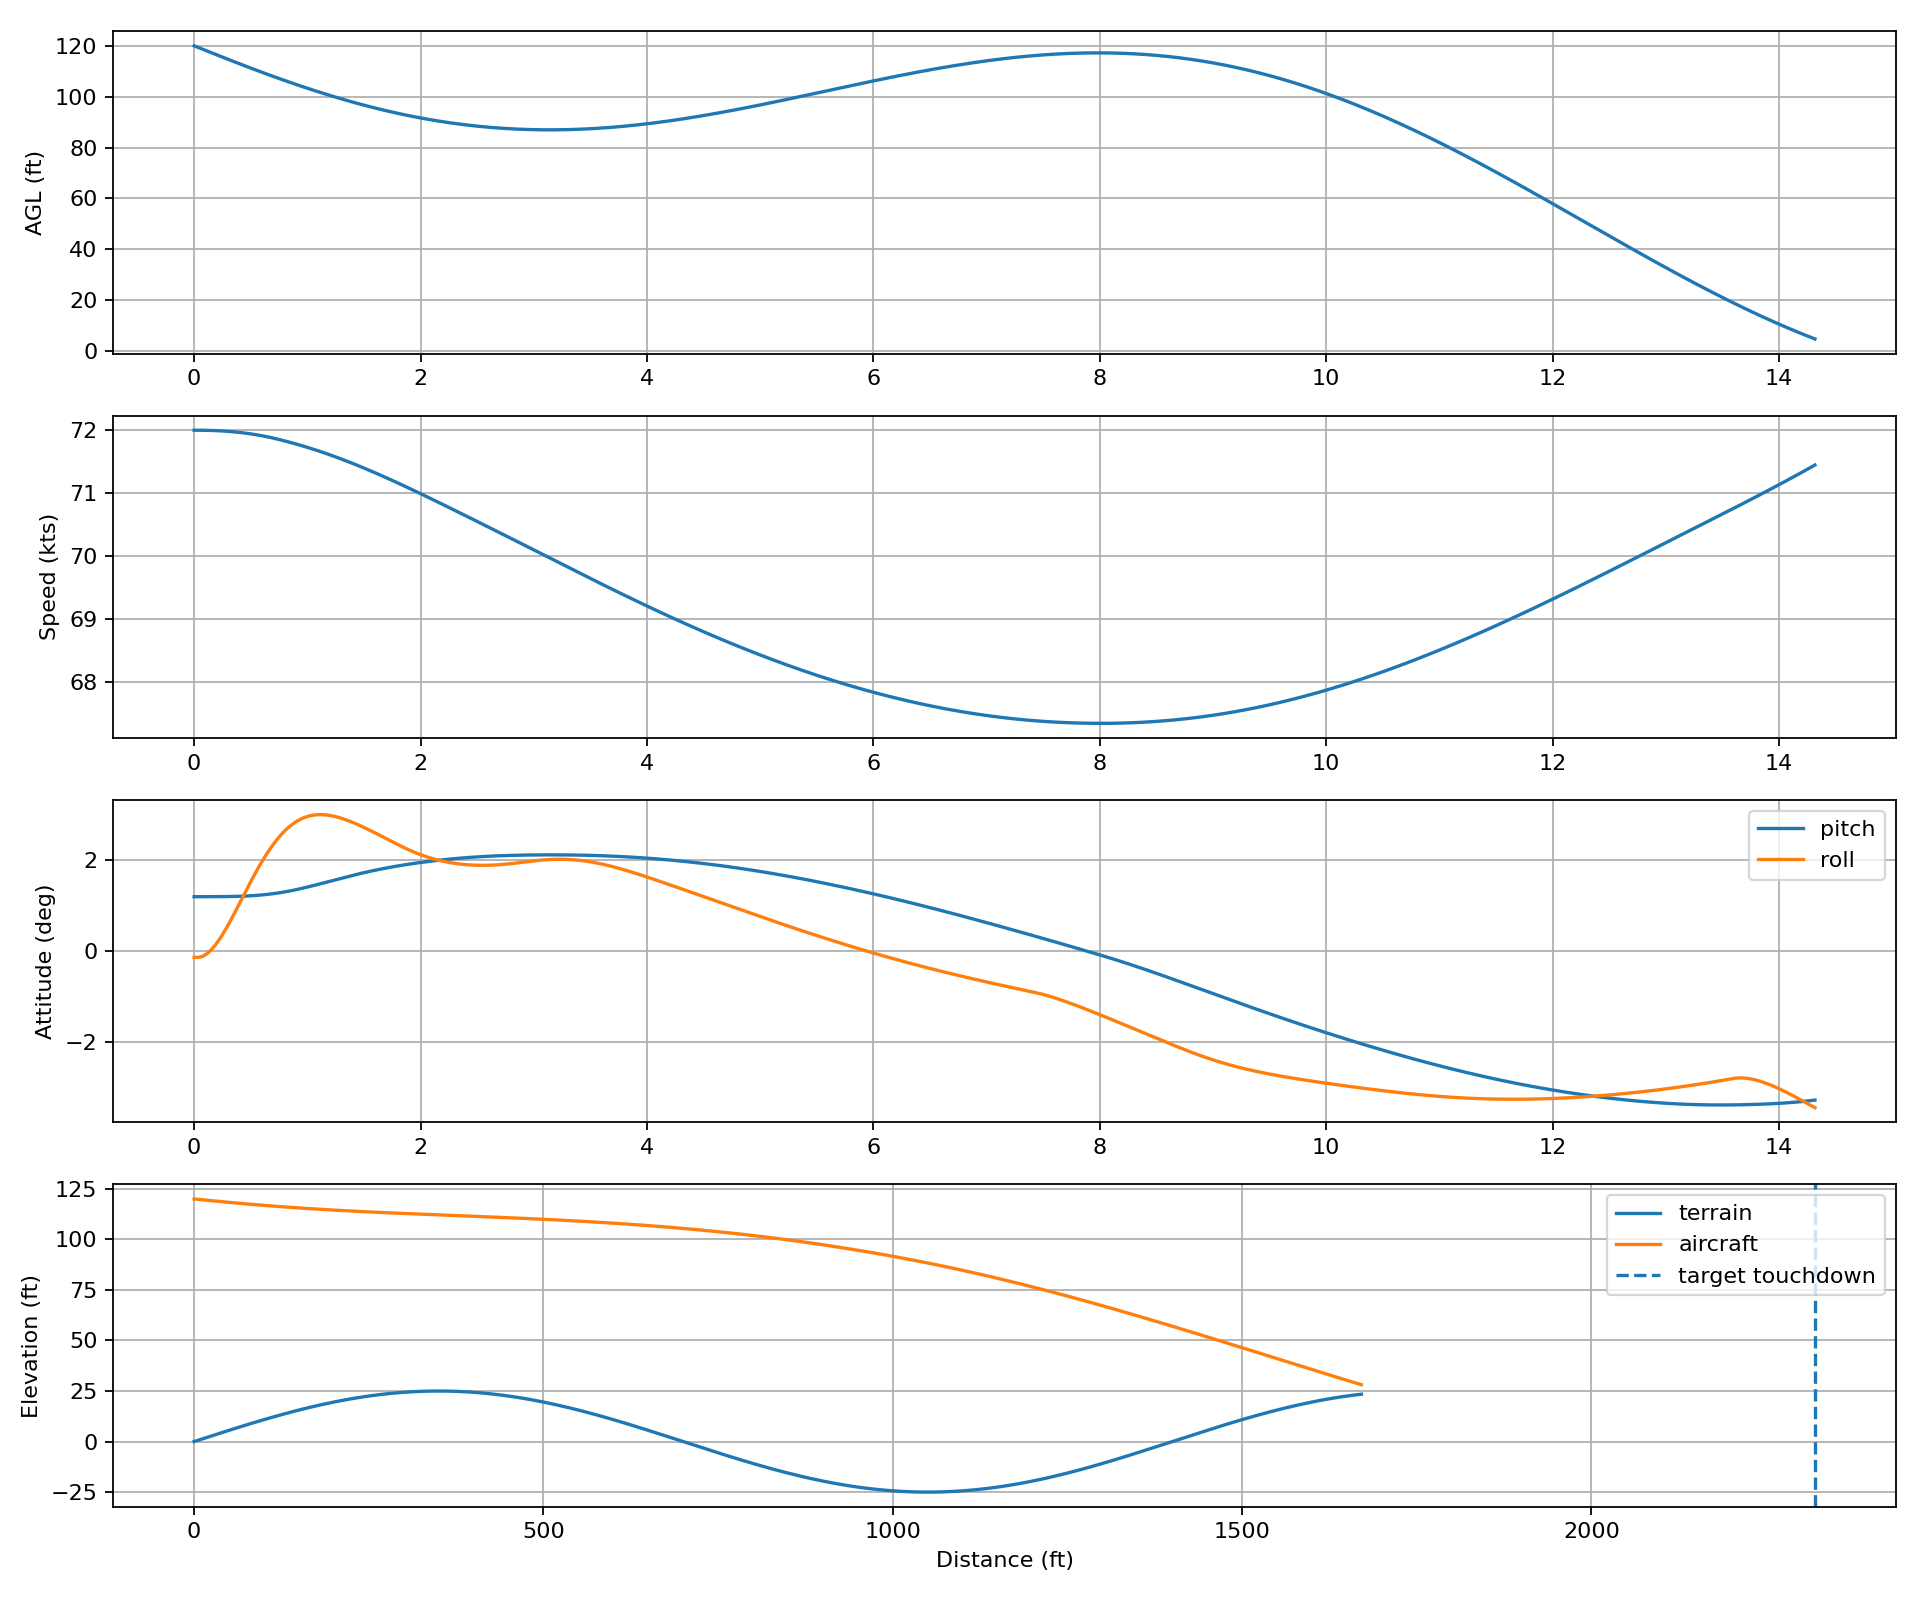
\includegraphics[width=3.47in,height=0.66\textheight,keepaspectratio]{images/image7.png}
\caption{基准工况模型校核结果图}
\label{fig:4-1}
\end{figure}

图~\ref{fig:4-1}反映了基准工况下飞行器AGL、速度、姿态角及轨迹变化情况。由图可见，飞行器在标准条件下状态收敛较好，说明模型校核结果满足后续分析要求。

\section{评价指标与判据建立}

为系统评价不同工况下固定翼飞行器着陆控制系统的性能，本文建立了评价指标模式，该模式包括安全性、稳定性、精度、交互有效性这四个方面。安全性指标包括飞行速度、最大下沉率、俯仰角与滚转角。稳定性指标涵盖离地高度变化是否连续、轨迹是否平滑、阶段切换是否合理。精度指标有侧偏量、航向误差、目标接地点附近位置的控制情况。交互有效性指标包括提示信息、告警触发、约束保护是否及时有效。

依据仿真平台的各项参数，本文确定了以下基本判据。在飞行速度处于62至88节这个范围，并且最大下沉率不超过850英尺每分钟，同时滚转角的绝对值不超过20度、俯仰角保持在负12度至16度之间的时候，判定系统符合基本飞行安全要求。当飞行器进入flare阶段之后，如果侧偏量不超过28英尺、航向误差不超过6度、滚转角不超过10度，那就判定拉平阶段横向对准状态良好。当进入接地提交阶段后，要是侧偏量不超过45英尺、航向误差不超过10度、滚转角不超过12度，便认为系统满足稳定接地要求。要是单项指标出现局部超限的情形，可判定为性能有所下降，要是多项关键指标同时超限，或者系统触发了复飞/中止逻辑，那么可判定为不利工况。

建立评价模式时，本文对着陆任务场景特点予以充分考虑。固定翼飞行器着陆属于典型的末段精确控制任务，仅靠单一指标不能全面展现系统性能，因此需把速度、姿态、侧偏及阶段切换等指标结合起来做综合评判。郑金豪在无人机精确着陆控制技术研究里指出，精确着陆的关键在于多状态量联合约束与分阶段控制协调。所以，本文建立的评价判据既关注单个状态量有无超出限定，也留意其在不同阶段的综合表现状况。

\begingroup\small
\begin{longtable}{@{}
  >{\raggedright\arraybackslash}p{(\columnwidth - 4\tabcolsep) * \real{0.3333}}
  >{\raggedright\arraybackslash}p{(\columnwidth - 4\tabcolsep) * \real{0.3334}}
  >{\raggedright\arraybackslash}p{(\columnwidth - 4\tabcolsep) * \real{0.3334}}@{}}
\caption{着陆性能评价指标与判据}\label{tab:4-1}\\
\toprule\noalign{}
\begin{minipage}[b]{\linewidth}\raggedright
指标类别
\end{minipage} & \begin{minipage}[b]{\linewidth}\raggedright
指标名称
\end{minipage} & \begin{minipage}[b]{\linewidth}\raggedright
判据
\end{minipage} \\
\midrule\noalign{}
\endhead
\bottomrule\noalign{}
\endlastfoot
安全性 & 飞行速度 & 62～88 kts \\
安全性 & 最大下沉率 & 不大于850 fpm \\
安全性 & 滚转角 & \textbar roll\textbar$\leq$20$^\circ$ \\
安全性 & 俯仰角 & -12$^\circ$～16$^\circ$ \\
精度 & flare阶段侧偏量 & $\leq$28 ft \\
精度 & flare阶段航向误差 & $\leq$6$^\circ$ \\
精度 & 接地提交侧偏量 & $\leq$45 ft \\
精度 & 接地提交航向误差 & $\leq$10$^\circ$ \\
稳定性 & 阶段切换 & 平滑、无明显突变 \\
交互有效性 & 告警与约束触发 & 及时、准确 \\
\end{longtable}
\endgroup

表~\ref{tab:4-1}给出了本文采用的主要评价指标与判据。后续各工况仿真结果均以该指标体系为基础进行横向比较和优劣识别。

\section{工况矩阵设计}

为剖析不同条件下模型的响应规律，本文依据已有的平台参数、仿真结果，设计了包括``地形条件
+ 控制模式 +
边界扰动''的工况矩阵。在地形条件这一方面，挑选了平坦地形、起伏地形、山脊地形、谷地地形、阶跃地形这五种具有代表性的环境，以此来呈现不同地面高程变化给着陆控制带来的影响，在控制模式上，设定了正常模式和保守模式这两种模式，用来探究不同目标速度策略下系统的性能差异，针对边界扰动，可以增加初始侧偏、航向误差或者较大下沉率等因素，从而建立更为复杂的工况场景。

在本文的基础工况里，主要是对五类地形展开对比，其他参数维持不变，以此来突出地形因素所产生的影响。为了验证控制系统对于不同进近地形扰动的适应能力，在本节当中设计了六类地形剖面，分别是平坦、起伏、山脊、谷地、阶跃、混合地形剖面，并且让初始高度保持在120英尺、速度维持在72节、跑道距离设定为2200英尺不变。将平坦地形用作基准参考，起伏地形用来分析连续高程变化对着地高度、姿态调节所造成的影响，山脊地形用于分析近地高程快速抬升时系统的应对状况，谷地地形用来分析先缓后急的相对离地高度变化情况，阶跃地形用于模拟局部高程突变对末段判断形成的干扰。借助这样的方式，便能够比较展现出不同场景下着陆控制系统的适应性能。

\begin{figure}[H]
\centering
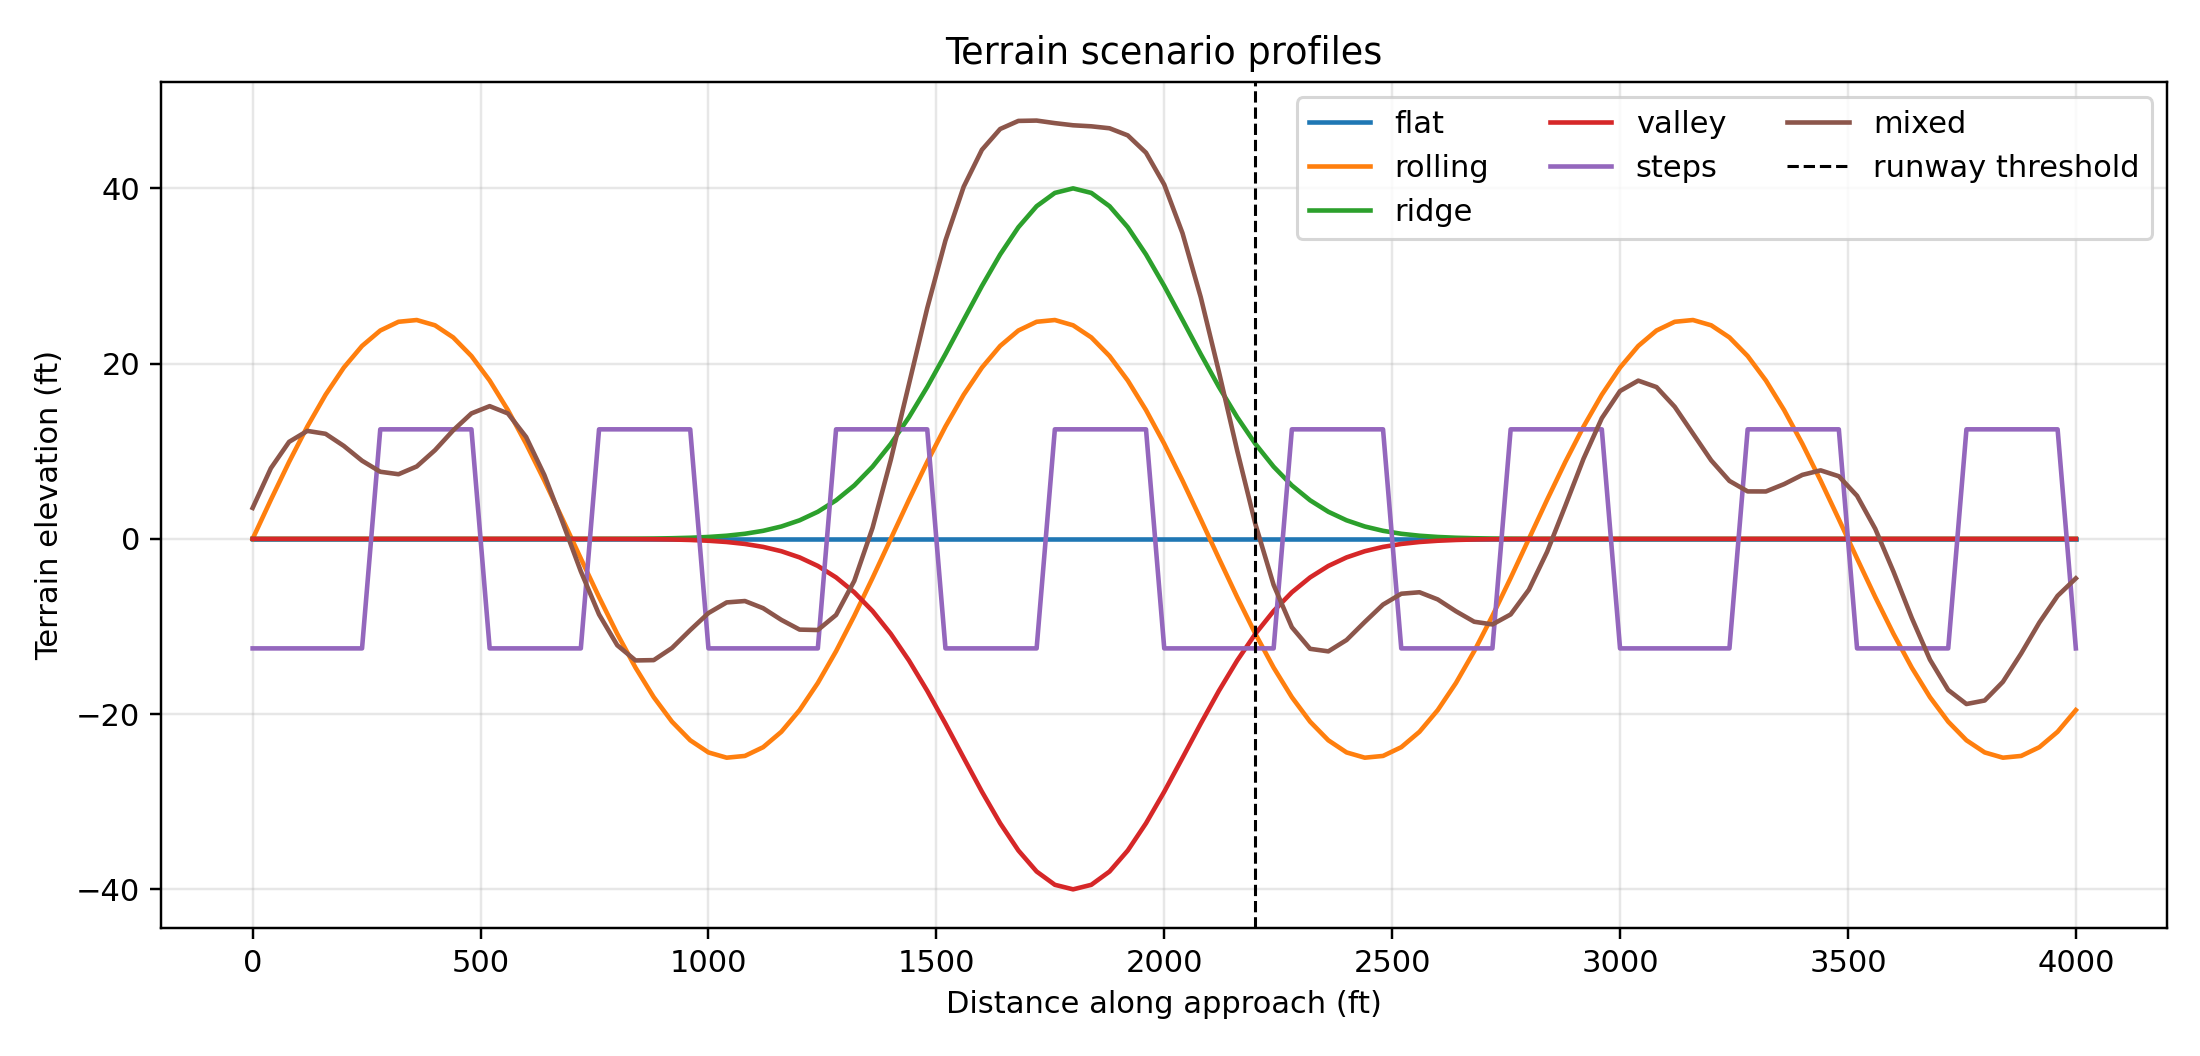
\includegraphics[width=0.92\linewidth,height=0.66\textheight,keepaspectratio]{images/image12.png}
\caption{不同地形工况的跑道进近剖面对比}
\label{fig:4-2}
\end{figure}

同时，为了体现工况设计的合理性，本文在矩阵设置中保留了由``标准条件''到``复杂条件''的渐进关系。先利用基础地形工况完成模型特性识别，再通过增加初始侧偏和下沉率偏差等方式扩展复杂工况。周乐等在仿生四足六旋翼无人机自适应着陆性能分析中指出，不同着陆场景对系统适应能力的要求具有明显差异，应通过多场景测试来识别系统的优势与薄弱环节。虽然本文对象为固定翼飞行器，但其工况设计思路同样适用，即通过典型场景组合提高评价的完整性。

\begingroup\small
\begin{longtable}{@{}
  >{\raggedright\arraybackslash}p{(\columnwidth - 10\tabcolsep) * \real{0.1666}}
  >{\raggedright\arraybackslash}p{(\columnwidth - 10\tabcolsep) * \real{0.1666}}
  >{\raggedright\arraybackslash}p{(\columnwidth - 10\tabcolsep) * \real{0.1666}}
  >{\raggedright\arraybackslash}p{(\columnwidth - 10\tabcolsep) * \real{0.1666}}
  >{\raggedright\arraybackslash}p{(\columnwidth - 10\tabcolsep) * \real{0.1667}}
  >{\raggedright\arraybackslash}p{(\columnwidth - 10\tabcolsep) * \real{0.1667}}@{}}
\caption{仿真工况矩阵设计}\label{tab:4-2}\\
\toprule\noalign{}
\begin{minipage}[b]{\linewidth}\raggedright
工况编号
\end{minipage} & \begin{minipage}[b]{\linewidth}\raggedright
地形类型
\end{minipage} & \begin{minipage}[b]{\linewidth}\raggedright
控制模式
\end{minipage} & \begin{minipage}[b]{\linewidth}\raggedright
初始侧偏
\end{minipage} & \begin{minipage}[b]{\linewidth}\raggedright
初始下降率
\end{minipage} & \begin{minipage}[b]{\linewidth}\raggedright
分析目标
\end{minipage} \\
\midrule\noalign{}
\endhead
\bottomrule\noalign{}
\endlastfoot
C1 & 平坦地形 & normal & 0 ft & -250 fpm & 基准工况校核 \\
C2 & 起伏地形 & normal & 0 ft & -250 fpm & 连续高程变化影响 \\
C3 & 山脊地形 & normal & 0 ft & -250 fpm & 近地抬升影响 \\
C4 & 谷地地形 & normal & 0 ft & -250 fpm & 谷地环境影响 \\
C5 & 阶跃地形 & normal & 0 ft & -250 fpm & 地形突变影响 \\
C6 & 平坦地形 & conservative & 0 ft & -250 fpm & 保守速度策略效果 \\
C7 & 起伏地形 & normal & 20 ft & -250 fpm & 横向偏差影响 \\
C8 & 山脊地形 & normal & 0 ft & -400 fpm & 较大下沉率影响 \\
\end{longtable}
\endgroup

\section{仿真计算与数据整理}

在工况矩阵确定完毕之后，本文运用统一的参数口径来进行仿真计算工作，并且借助CSV导出、曲线图绘制的方式对结果加以整理。仿真输出所涵盖的内容主要有时间、飞行距离、跑道相对距离、目标接地点距离、离地高度、海拔高度、速度、下沉率、俯仰角、滚转角、航向角、侧偏量、控制指令、飞行阶段、提示与告警信息等。对这些数据予以整理之后，能够进一步提取出各工况下的末段速度、末段姿态、末段离地高度、阶段切换特征。

根据已有的基础工况成果，五类地形的主要数据情况是这样的。平坦地形工况下，仿真时长为十七点一五秒，末端的AGL大约是四点六零英尺，末端速度约为七十一点八零节。起伏地形工况的仿真时长为十四点三二秒，末端AGL约为四点七零英尺，末端速度约为七十一点四五节。山脊地形工况的仿真时长是十四点零三秒，末端AGL约为四点七四英尺，末端速度约为七十点四四节。谷地地形工况的仿真时长为十八点四七秒，末端AGL约是四点六零英尺，末端速度约为七十一点七八节。阶跃地形工况的仿真时长是十五点零二秒，末端AGL约为一点二零英尺，末端速度约为七十点九四节。从这些数据可以发现，不同地形状况下系统的输出有差别，其中阶跃地形对近地高度的判断影响较大，起伏地形和山脊地形对姿态修正、末端控制的影响比较明显。

\begingroup\small
\begin{longtable}{@{}
  >{\raggedright\arraybackslash}p{(\columnwidth - 10\tabcolsep) * \real{0.1666}}
  >{\raggedright\arraybackslash}p{(\columnwidth - 10\tabcolsep) * \real{0.1666}}
  >{\raggedright\arraybackslash}p{(\columnwidth - 10\tabcolsep) * \real{0.1666}}
  >{\raggedright\arraybackslash}p{(\columnwidth - 10\tabcolsep) * \real{0.1666}}
  >{\raggedright\arraybackslash}p{(\columnwidth - 10\tabcolsep) * \real{0.1667}}
  >{\raggedright\arraybackslash}p{(\columnwidth - 10\tabcolsep) * \real{0.1667}}@{}}
\caption{不同地形基础工况关键结果整理}\label{tab:4-3}\\
\toprule\noalign{}
\begin{minipage}[b]{\linewidth}\raggedright
地形工况
\end{minipage} & \begin{minipage}[b]{\linewidth}\raggedright
仿真时长/s
\end{minipage} & \begin{minipage}[b]{\linewidth}\raggedright
末段AGL/ft
\end{minipage} & \begin{minipage}[b]{\linewidth}\raggedright
末段速度/kts
\end{minipage} & \begin{minipage}[b]{\linewidth}\raggedright
末段俯仰角/($^\circ$)
\end{minipage} & \begin{minipage}[b]{\linewidth}\raggedright
末段滚转角/($^\circ$)
\end{minipage} \\
\midrule\noalign{}
\endhead
\bottomrule\noalign{}
\endlastfoot
平坦地形 & 17.15 & 4.60 & 71.80 & -1.28 & -2.28 \\
起伏地形 & 14.32 & 4.70 & 71.45 & -3.29 & -3.45 \\
山脊地形 & 14.03 & 4.74 & 70.44 & -2.52 & -2.96 \\
谷地地形 & 18.47 & 4.60 & 71.78 & -0.90 & 2.09 \\
阶跃地形 & 15.02 & 1.20 & 70.94 & -2.33 & -3.67 \\
\end{longtable}
\endgroup

由表~\ref{tab:4-3}可以看出，不同地形条件下系统输出存在明显差异。其中，起伏地形和山脊地形使飞行器姿态修正幅度更大，谷地地形使仿真持续时间相对较长，而阶跃地形对末段离地高度影响最突出。这些结果表明，本文所建立的模型和仿真平台能够较好地区分不同工况下的着陆响应差异，并为后续第5章``不利工况识别与机理解释''提供数据基础。
